%************************************************
\chapter{Hydrogen Balmer Series and Rydberg Constant}
%************************************************
\begin{flushright}
Feb 19 and 26, 2013
\end{flushright}
\section{Aim}
	To experimentally measure the Balmer series line of the Hydrogen spectrum and calculate Rydberg's constant, $R$ from the result.
\section{Apparatus}
	Hydrogen Discharge tube, Diffraction grating, Spectroscope

\section{Theory}
	\subsection{Motivation}
		The Spectrum of hydrogen is spread over a large range in the electromagnetic spectrum. The visible part is known as the Balmer series, given by the formula
		\begin{equation}
			\frac 1 \lambda = R \left[ \frac 1 4 - \frac 1 {n^2} \right]
		\end{equation}
		where n is an integer > 2. The general formula for the Hydrogen Spectra is given by
		\begin{equation}
			\frac 1 \lambda = R \left[ \frac 1 {n_f^2}  - \frac 1 {n_i^2} \right]
		\end{equation}
		where $n_f>n_i$. This reduces to the previous formula for $n_f=2$. This equation was derived by Rydberg as a phenomenological description. The same equation was derived by Bohr, from more basic principles of physics, using quantization ideas from Plank and Einstein, and certain other bold assumptions (no radiation for specific orbits and angular momenta) to conclude the following
		\begin{equation}
			R = \frac {me^4} {8\epsilon_0^2 h^3 c}
		\end{equation}
		where m and c are mass and charge of the electron
	\subsection{Experimental Setup}	
		The setup is fairly straight forward. We have a Hydrogen discharge tube (source of Hydrogen spectrum) placed in front of a [[telescope device]] with a diffraction grating in between. This grating results in splitting of the spectrum spatially. We measure the positions of these split lines to find their wavelengths and plot the corresponding quantities to find the value of R.
	\subsection{Useful Results}
		To calculate $\lambda$, we use the relation $d \sin \theta = m \lambda$ with $m = 1$.
		\par
		R in SI units is $1.09 \times 10^7 m^{-1}$
		\par
		The wavelengths of the Balmer series are 656.28 nm, 486.13 nm, 434.05 nm and 410.17 nm, for $n = 3, 4, 5,$ and $6$ respectively.
\section{Observations and Calculations}
	Please refer to \autoref{e3_result}. The Rydberg's constant was determined to be $1.00 \times 10^{7}$ with $R^2=0.9213$ for the straight line fit.

	% \begin{figure}[bth]
	% 	\begin{center}
	% 		
\includegraphics[width=1.0\linewidth]{gfx/e2_circuit}
	% 	\end{center}
	% \caption[Simplified schematic of the Setup]{Simplified schematic of the Setup}
	% \label{e2_circuit}
	% \end{figure}	

\section{Procedure}
	The procedure has been influenced heavily by the one given in the Physics Lab Manual, provided to us, during the course, PHY212, 2013.
	\begin{enumerate}
		\item Focussed the telescope to infinity (Took the telescope outside the dark room for this, focussed at something outside the window)
		\item Placed the light source about 1 cm from the collimator slit. The slit was left barely open.
		\item Looked through the eye piece and adjusted it to ensure the cross wire is aligned well and visible. Do NOT move the telescope's focus
		\item Rotated the telescope arm to align directly with the collimator.
		\item Turned on the light source and viewed the slit of the collimator
		\item Focussed the collimator to obtain a sharp image of the slit.
		\item Now placed the diffraction grating in the corresponding mount, at right angles to the axis formed by the collimator and the telescope
		\item Looked straight through the telescope to continue seeing the direct image of the slit. Ensure at this stage that the image is getting formed at the centre.
		\item Used the cross wire to measure the left and right edge of the slit
		\item Rotated the arm of the telescope to left or right, and observed the coloured spectrum. The contrast of the lines can be increased at the cost of brightness by adjusting the slit width. This may be done to identify the first order lines. Higher order lines come at higher angular deviations.
		\item Noted the position of the three Balmer lines corresponding to $n_i=5,4$ and 3.
	\end{enumerate}

\section{Result}
	The expected value of the Rydberg constant $R=1.09 \times 10^7 m^{-1}$. Experimentally this was determined to be $(1.00 \pm 0.078) \times 10^{7}$ ($R^2=0.9213$ for the straight line fit whose slope is the Rydberg's constant).

	\clearpage
	\begin{figure}[bth]
		\begin{center}
			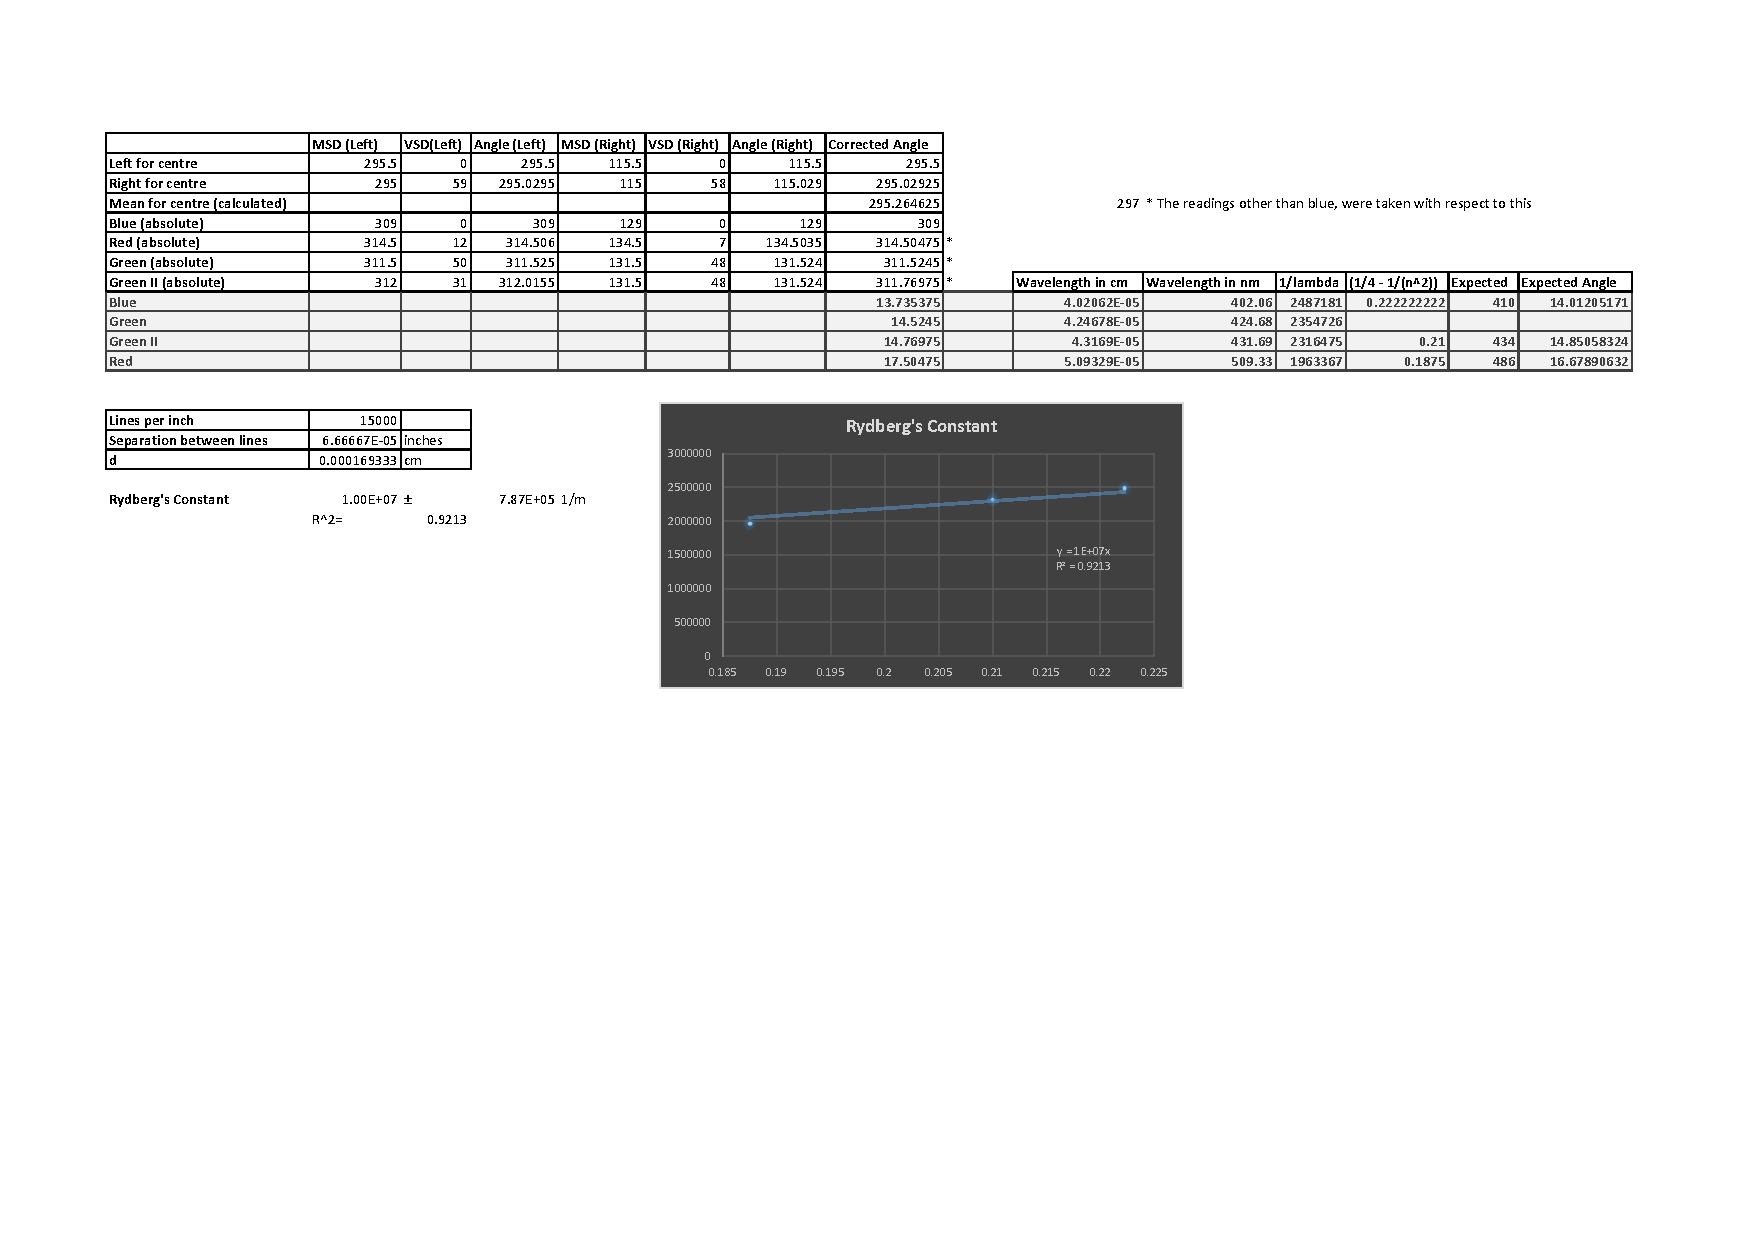
\includegraphics[width=1.3\linewidth]{gfx/exp3.pdf}
		\end{center}
	\caption[Observations for Frank-Hertz]{Observations for Frank-Hertz}
	\label{e3_result}
	\end{figure}
